\section{Register description}
\regover{
{\hyperref[sec_eng-se-sha-0-ctrl]{se\_sha\_0\_ctrl}}&
\\
\hline
{\hyperref[sec_eng-se-sha-0-msa]{se\_sha\_0\_msa}}&
\\
\hline
{\hyperref[sec_eng-se-sha-0-status]{se\_sha\_0\_status}}&
\\
\hline
{\hyperref[sec_eng-se-sha-0-endian]{se\_sha\_0\_endian}}&
\\
\hline
{\hyperref[sec_eng-se-sha-0-hash-l-0]{se\_sha\_0\_hash\_l\_0}}&
\\
\hline
{\hyperref[sec_eng-se-sha-0-hash-l-1]{se\_sha\_0\_hash\_l\_1}}&
\\
\hline
{\hyperref[sec_eng-se-sha-0-hash-l-2]{se\_sha\_0\_hash\_l\_2}}&
\\
\hline
{\hyperref[sec_eng-se-sha-0-hash-l-3]{se\_sha\_0\_hash\_l\_3}}&
\\
\hline
{\hyperref[sec_eng-se-sha-0-hash-l-4]{se\_sha\_0\_hash\_l\_4}}&
\\
\hline
{\hyperref[sec_eng-se-sha-0-hash-l-5]{se\_sha\_0\_hash\_l\_5}}&
\\
\hline
{\hyperref[sec_eng-se-sha-0-hash-l-6]{se\_sha\_0\_hash\_l\_6}}&
\\
\hline
{\hyperref[sec_eng-se-sha-0-hash-l-7]{se\_sha\_0\_hash\_l\_7}}&
\\
\hline
{\hyperref[sec_eng-se-sha-0-hash-h-0]{se\_sha\_0\_hash\_h\_0}}&
\\
\hline
{\hyperref[sec_eng-se-sha-0-hash-h-1]{se\_sha\_0\_hash\_h\_1}}&
\\
\hline
{\hyperref[sec_eng-se-sha-0-hash-h-2]{se\_sha\_0\_hash\_h\_2}}&
\\
\hline
{\hyperref[sec_eng-se-sha-0-hash-h-3]{se\_sha\_0\_hash\_h\_3}}&
\\
\hline
{\hyperref[sec_eng-se-sha-0-hash-h-4]{se\_sha\_0\_hash\_h\_4}}&
\\
\hline
{\hyperref[sec_eng-se-sha-0-hash-h-5]{se\_sha\_0\_hash\_h\_5}}&
\\
\hline
{\hyperref[sec_eng-se-sha-0-hash-h-6]{se\_sha\_0\_hash\_h\_6}}&
\\
\hline
{\hyperref[sec_eng-se-sha-0-hash-h-7]{se\_sha\_0\_hash\_h\_7}}&
\\
\hline
{\hyperref[sec_eng-se-sha-0-link]{se\_sha\_0\_link}}&
\\
\hline
{\hyperref[sec_eng-se-sha-0-ctrl-prot]{se\_sha\_0\_ctrl\_prot}}&
\\
\hline
{\hyperref[sec_eng-se-aes-0-ctrl]{se\_aes\_0\_ctrl}}&
\\
\hline
{\hyperref[sec_eng-se-aes-0-msa]{se\_aes\_0\_msa}}&
\\
\hline
{\hyperref[sec_eng-se-aes-0-mda]{se\_aes\_0\_mda}}&
\\
\hline
{\hyperref[sec_eng-se-aes-0-status]{se\_aes\_0\_status}}&
\\
\hline
{\hyperref[sec_eng-se-aes-0-iv-0]{se\_aes\_0\_iv\_0}}&
\\
\hline
{\hyperref[sec_eng-se-aes-0-iv-1]{se\_aes\_0\_iv\_1}}&
\\
\hline
{\hyperref[sec_eng-se-aes-0-iv-2]{se\_aes\_0\_iv\_2}}&
\\
\hline
{\hyperref[sec_eng-se-aes-0-iv-3]{se\_aes\_0\_iv\_3}}&
\\
\hline
{\hyperref[sec_eng-se-aes-0-key-0]{se\_aes\_0\_key\_0}}&
\\
\hline
{\hyperref[sec_eng-se-aes-0-key-1]{se\_aes\_0\_key\_1}}&
\\
\hline
{\hyperref[sec_eng-se-aes-0-key-2]{se\_aes\_0\_key\_2}}&
\\
\hline
{\hyperref[sec_eng-se-aes-0-key-3]{se\_aes\_0\_key\_3}}&
\\
\hline
{\hyperref[sec_eng-se-aes-0-key-4]{se\_aes\_0\_key\_4}}&
\\
\hline
{\hyperref[sec_eng-se-aes-0-key-5]{se\_aes\_0\_key\_5}}&
\\
\hline
{\hyperref[sec_eng-se-aes-0-key-6]{se\_aes\_0\_key\_6}}&
\\
\hline
{\hyperref[sec_eng-se-aes-0-key-7]{se\_aes\_0\_key\_7}}&
\\
\hline
{\hyperref[sec_eng-se-aes-0-key-sel]{se\_aes\_0\_key\_sel}}&
\\
\hline
{\hyperref[sec_eng-se-aes-1-key-sel]{se\_aes\_1\_key\_sel}}&
\\
\hline
{\hyperref[sec_eng-se-aes-0-endian]{se\_aes\_0\_endian}}&
\\
\hline
{\hyperref[sec_eng-se-aes-sboot]{se\_aes\_sboot}}&
\\
\hline
{\hyperref[sec_eng-se-aes-0-link]{se\_aes\_0\_link}}&
\\
\hline
{\hyperref[sec_eng-se-aes-0-ctrl-prot]{se\_aes\_0\_ctrl\_prot}}&
\\
\hline
{\hyperref[sec_eng-se-trng-0-ctrl-0]{se\_trng\_0\_ctrl\_0}}&
\\
\hline
{\hyperref[sec_eng-se-trng-0-status]{se\_trng\_0\_status}}&
\\
\hline
{\hyperref[sec_eng-se-trng-0-dout-0]{se\_trng\_0\_dout\_0}}&
\\
\hline
{\hyperref[sec_eng-se-trng-0-dout-1]{se\_trng\_0\_dout\_1}}&
\\
\hline
{\hyperref[sec_eng-se-trng-0-dout-2]{se\_trng\_0\_dout\_2}}&
\\
\hline
{\hyperref[sec_eng-se-trng-0-dout-3]{se\_trng\_0\_dout\_3}}&
\\
\hline
{\hyperref[sec_eng-se-trng-0-dout-4]{se\_trng\_0\_dout\_4}}&
\\
\hline
{\hyperref[sec_eng-se-trng-0-dout-5]{se\_trng\_0\_dout\_5}}&
\\
\hline
{\hyperref[sec_eng-se-trng-0-dout-6]{se\_trng\_0\_dout\_6}}&
\\
\hline
{\hyperref[sec_eng-se-trng-0-dout-7]{se\_trng\_0\_dout\_7}}&
\\
\hline
{\hyperref[sec_eng-se-trng-0-test]{se\_trng\_0\_test}}&
\\
\hline
{\hyperref[sec_eng-se-trng-0-ctrl-1]{se\_trng\_0\_ctrl\_1}}&
\\
\hline
{\hyperref[sec_eng-se-trng-0-ctrl-2]{se\_trng\_0\_ctrl\_2}}&
\\
\hline
{\hyperref[sec_eng-se-trng-0-ctrl-3]{se\_trng\_0\_ctrl\_3}}&
\\
\hline
{\hyperref[sec_eng-se-trng-0-test-out-0]{se\_trng\_0\_test\_out\_0}}&
\\
\hline
{\hyperref[sec_eng-se-trng-0-test-out-1]{se\_trng\_0\_test\_out\_1}}&
\\
\hline
{\hyperref[sec_eng-se-trng-0-test-out-2]{se\_trng\_0\_test\_out\_2}}&
\\
\hline
{\hyperref[sec_eng-se-trng-0-test-out-3]{se\_trng\_0\_test\_out\_3}}&
\\
\hline
{\hyperref[sec_eng-se-trng-0-ctrl-prot]{se\_trng\_0\_ctrl\_prot}}&
\\
\hline
{\hyperref[sec_eng-se-pka-0-ctrl-0]{se\_pka\_0\_ctrl\_0}}&
\\
\hline
{\hyperref[sec_eng-se-pka-0-seed]{se\_pka\_0\_seed}}&
\\
\hline
{\hyperref[sec_eng-se-pka-0-ctrl-1]{se\_pka\_0\_ctrl\_1}}&
\\
\hline
{\hyperref[sec_eng-se-pka-0-rw]{se\_pka\_0\_rw}}&
\\
\hline
{\hyperref[sec_eng-se-pka-0-rw-burst]{se\_pka\_0\_rw\_burst}}&
\\
\hline
{\hyperref[sec_eng-se-pka-0-ctrl-prot]{se\_pka\_0\_ctrl\_prot}}&
\\
\hline
{\hyperref[sec_eng-se-cdet-0-ctrl-0]{se\_cdet\_0\_ctrl\_0}}&
\\
\hline
{\hyperref[sec_eng-se-cdet-0-ctrl-1]{se\_cdet\_0\_ctrl\_1}}&
\\
\hline
{\hyperref[sec_eng-se-cdet-0-ctrl-2]{se\_cdet\_0\_ctrl\_2}}&
\\
\hline
{\hyperref[sec_eng-se-cdet-0-ctrl-3]{se\_cdet\_0\_ctrl\_3}}&
\\
\hline
{\hyperref[sec_eng-se-cdet-0-ctrl-prot]{se\_cdet\_0\_ctrl\_prot}}&
\\
\hline
{\hyperref[sec_eng-se-gmac-0-ctrl-0]{se\_gmac\_0\_ctrl\_0}}&
\\
\hline
{\hyperref[sec_eng-se-gmac-0-lca]{se\_gmac\_0\_lca}}&
\\
\hline
{\hyperref[sec_eng-se-gmac-0-status]{se\_gmac\_0\_status}}&
\\
\hline
{\hyperref[sec_eng-se-gmac-0-ctrl-prot]{se\_gmac\_0\_ctrl\_prot}}&
\\
\hline
{\hyperref[sec_eng-se-ctrl-prot-rd]{se\_ctrl\_prot\_rd}}&
\\
\hline
{\hyperref[sec_eng-se-ctrl-reserved-0]{se\_ctrl\_reserved\_0}}&
\\
\hline
{\hyperref[sec_eng-se-ctrl-reserved-1]{se\_ctrl\_reserved\_1}}&
\\
\hline
{\hyperref[sec_eng-se-ctrl-reserved-2]{se\_ctrl\_reserved\_2}}&
\\
\hline
}

\subsection{se\_sha\_0\_ctrl}
\label{sec_eng-se-sha-0-ctrl}
Address:0x20004000
 \begin{figure}[H]
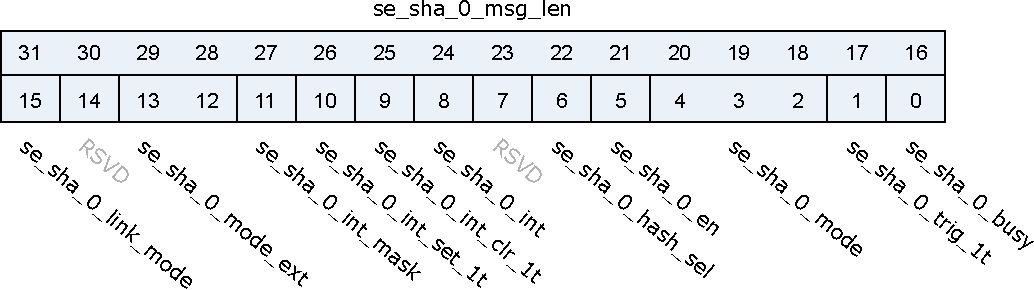
\includegraphics{sec_eng_se_sha_0_ctrl.pdf}
\end{figure}

\regdes{31:16&se\_sha\_0\_msg\_len&r/w&0&number of 512-bit block\\\hline
15&se\_sha\_0\_link\_mode&r/w&0&1:enable sha link mode\\\hline
14&RSVD& & & \\\hline
13:12&se\_sha\_0\_mode\_ext&r/w&0&hash mode extention; 0:SHA 1:MD5 2:CRC-16 3:CRC-32\\\hline
11&se\_sha\_0\_int\_mask&r/w&0&\\\hline
10&se\_sha\_0\_int\_set\_1t&w1p&0&1:set interrupt\\\hline
9&se\_sha\_0\_int\_clr\_1t&w1p&0&1:clear interrupt\\\hline
8&se\_sha\_0\_int&r&0&interrupt value\\\hline
7&RSVD& & & \\\hline
6&se\_sha\_0\_hash\_sel&r/w&0&0:new hash 1:accumulate last hash\\\hline
5&se\_sha\_0\_en&r/w&0&1:enable sha engine\\\hline
4:2&se\_sha\_0\_mode&r/w&0&0:SHA-256 1:SHA-224 2:SHA-1 3:SHA-1 4:SHA-512 5:SHA-384 6:SHA-512/224 7:SHA-512/256\\\hline
1&se\_sha\_0\_trig\_1t&w1p&0&1:trigger sha engine\\\hline
0&se\_sha\_0\_busy&r&0&1:sha engine busy\\\hline

}
\subsection{se\_sha\_0\_msa}
\label{sec_eng-se-sha-0-msa}
Address:0x20004004
 \begin{figure}[H]
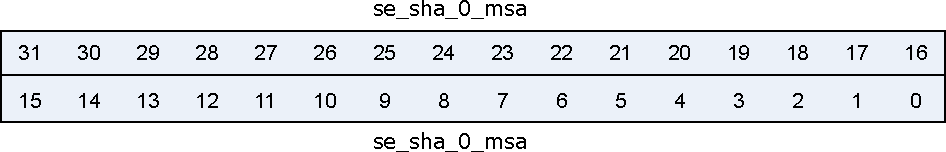
\includegraphics{sec_eng_se_sha_0_msa.pdf}
\end{figure}

\regdes{31:0&se\_sha\_0\_msa&r/w&0&message source address\\\hline

}
\subsection{se\_sha\_0\_status}
\label{sec_eng-se-sha-0-status}
Address:0x20004008
 \begin{figure}[H]
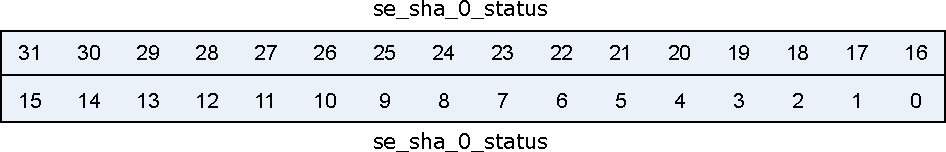
\includegraphics{sec_eng_se_sha_0_status.pdf}
\end{figure}

\regdes{31:0&se\_sha\_0\_status&r&32'h41&\\\hline

}
\subsection{se\_sha\_0\_endian}
\label{sec_eng-se-sha-0-endian}
Address:0x2000400c
 \begin{figure}[H]
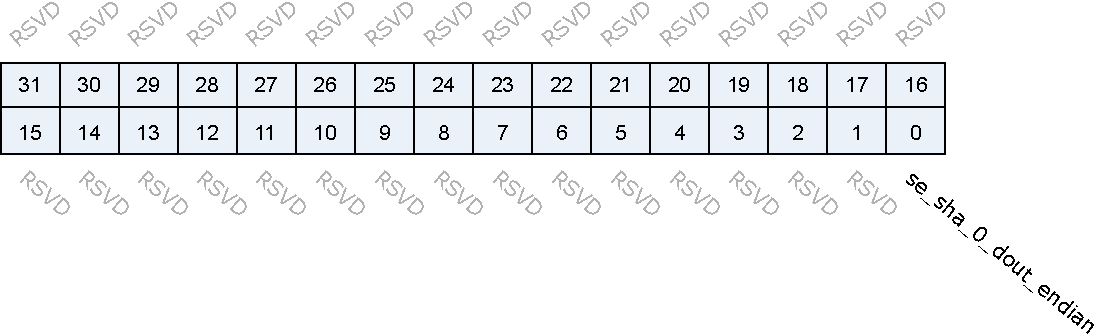
\includegraphics{sec_eng_se_sha_0_endian.pdf}
\end{figure}

\regdes{31:1&RSVD& & & \\\hline
0&se\_sha\_0\_dout\_endian&r/w&1&0:little-endian 1:big-endian\\\hline

}
\subsection{se\_sha\_0\_hash\_l\_0}
\label{sec_eng-se-sha-0-hash-l-0}
Address:0x20004010
 \begin{figure}[H]
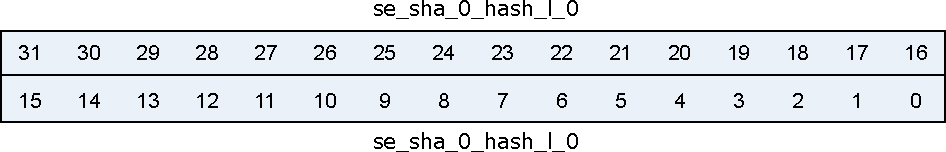
\includegraphics{sec_eng_se_sha_0_hash_l_0.pdf}
\end{figure}

\regdes{31:0&se\_sha\_0\_hash\_l\_0&r&0&big-endian hash 0 (MSB)\\\hline

}
\subsection{se\_sha\_0\_hash\_l\_1}
\label{sec_eng-se-sha-0-hash-l-1}
Address:0x20004014
 \begin{figure}[H]
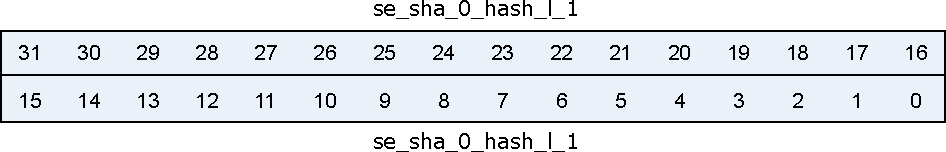
\includegraphics{sec_eng_se_sha_0_hash_l_1.pdf}
\end{figure}

\regdes{31:0&se\_sha\_0\_hash\_l\_1&r&0&big-endian hash 1\\\hline

}
\subsection{se\_sha\_0\_hash\_l\_2}
\label{sec_eng-se-sha-0-hash-l-2}
Address:0x20004018
 \begin{figure}[H]
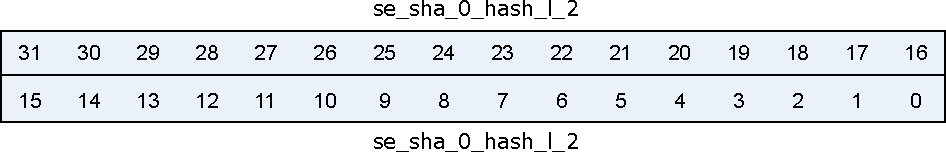
\includegraphics{sec_eng_se_sha_0_hash_l_2.pdf}
\end{figure}

\regdes{31:0&se\_sha\_0\_hash\_l\_2&r&0&big-endian hash 2\\\hline

}
\subsection{se\_sha\_0\_hash\_l\_3}
\label{sec_eng-se-sha-0-hash-l-3}
Address:0x2000401c
 \begin{figure}[H]
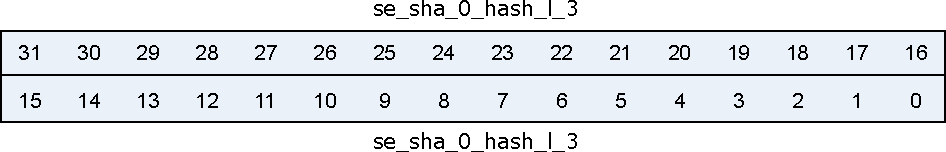
\includegraphics{sec_eng_se_sha_0_hash_l_3.pdf}
\end{figure}

\regdes{31:0&se\_sha\_0\_hash\_l\_3&r&0&big-endian hash 3\\\hline

}
\subsection{se\_sha\_0\_hash\_l\_4}
\label{sec_eng-se-sha-0-hash-l-4}
Address:0x20004020
 \begin{figure}[H]
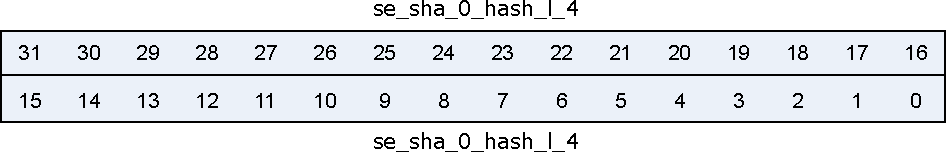
\includegraphics{sec_eng_se_sha_0_hash_l_4.pdf}
\end{figure}

\regdes{31:0&se\_sha\_0\_hash\_l\_4&r&0&big-endian hash 4\\\hline

}
\subsection{se\_sha\_0\_hash\_l\_5}
\label{sec_eng-se-sha-0-hash-l-5}
Address:0x20004024
 \begin{figure}[H]
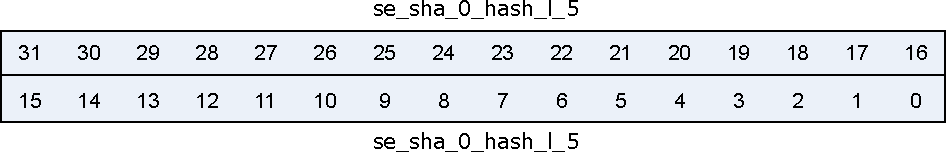
\includegraphics{sec_eng_se_sha_0_hash_l_5.pdf}
\end{figure}

\regdes{31:0&se\_sha\_0\_hash\_l\_5&r&0&big-endian hash 5\\\hline

}
\subsection{se\_sha\_0\_hash\_l\_6}
\label{sec_eng-se-sha-0-hash-l-6}
Address:0x20004028
 \begin{figure}[H]
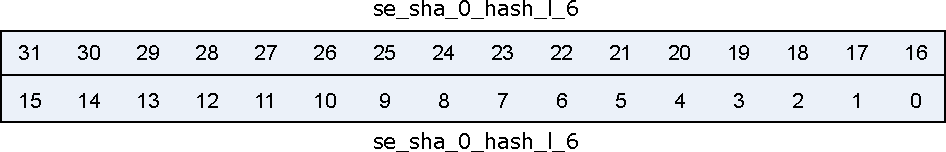
\includegraphics{sec_eng_se_sha_0_hash_l_6.pdf}
\end{figure}

\regdes{31:0&se\_sha\_0\_hash\_l\_6&r&0&big-endian hash 6\\\hline

}
\subsection{se\_sha\_0\_hash\_l\_7}
\label{sec_eng-se-sha-0-hash-l-7}
Address:0x2000402c
 \begin{figure}[H]
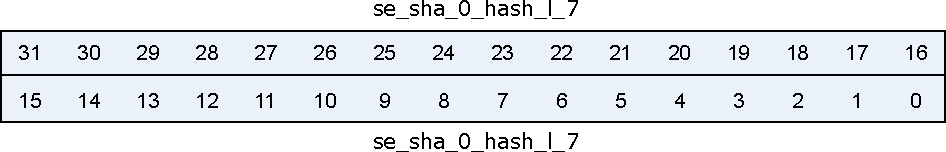
\includegraphics{sec_eng_se_sha_0_hash_l_7.pdf}
\end{figure}

\regdes{31:0&se\_sha\_0\_hash\_l\_7&r&0&big-endian hash 7 (LSB)\\\hline

}
\subsection{se\_sha\_0\_hash\_h\_0}
\label{sec_eng-se-sha-0-hash-h-0}
Address:0x20004030
 \begin{figure}[H]
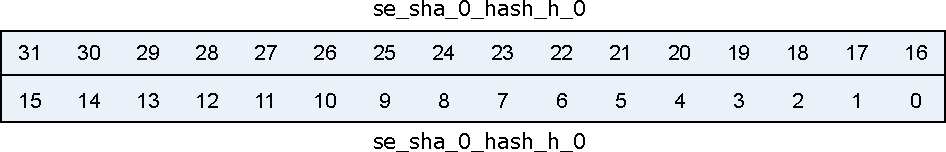
\includegraphics{sec_eng_se_sha_0_hash_h_0.pdf}
\end{figure}

\regdes{31:0&se\_sha\_0\_hash\_h\_0&r&0&big-endian hash 0 (MSB)\\\hline

}
\subsection{se\_sha\_0\_hash\_h\_1}
\label{sec_eng-se-sha-0-hash-h-1}
Address:0x20004034
 \begin{figure}[H]
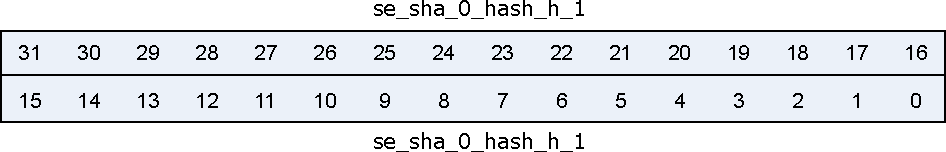
\includegraphics{sec_eng_se_sha_0_hash_h_1.pdf}
\end{figure}

\regdes{31:0&se\_sha\_0\_hash\_h\_1&r&0&big-endian hash 1\\\hline

}
\subsection{se\_sha\_0\_hash\_h\_2}
\label{sec_eng-se-sha-0-hash-h-2}
Address:0x20004038
 \begin{figure}[H]
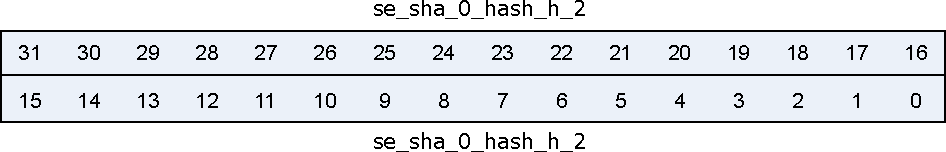
\includegraphics{sec_eng_se_sha_0_hash_h_2.pdf}
\end{figure}

\regdes{31:0&se\_sha\_0\_hash\_h\_2&r&0&big-endian hash 2\\\hline

}
\subsection{se\_sha\_0\_hash\_h\_3}
\label{sec_eng-se-sha-0-hash-h-3}
Address:0x2000403c
 \begin{figure}[H]
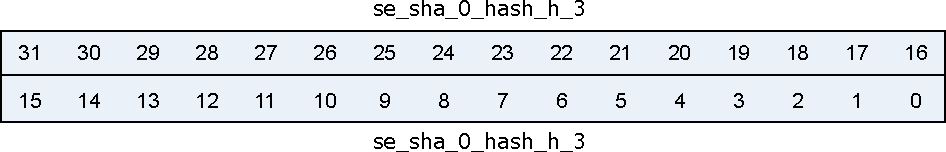
\includegraphics{sec_eng_se_sha_0_hash_h_3.pdf}
\end{figure}

\regdes{31:0&se\_sha\_0\_hash\_h\_3&r&0&big-endian hash 3\\\hline

}
\subsection{se\_sha\_0\_hash\_h\_4}
\label{sec_eng-se-sha-0-hash-h-4}
Address:0x20004040
 \begin{figure}[H]
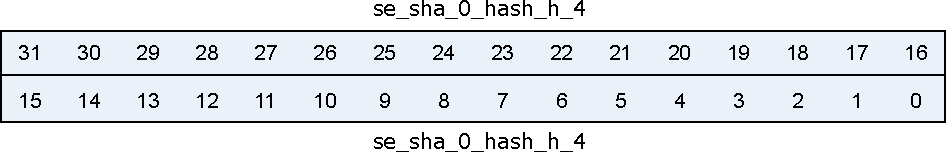
\includegraphics{sec_eng_se_sha_0_hash_h_4.pdf}
\end{figure}

\regdes{31:0&se\_sha\_0\_hash\_h\_4&r&0&big-endian hash 4\\\hline

}
\subsection{se\_sha\_0\_hash\_h\_5}
\label{sec_eng-se-sha-0-hash-h-5}
Address:0x20004044
 \begin{figure}[H]
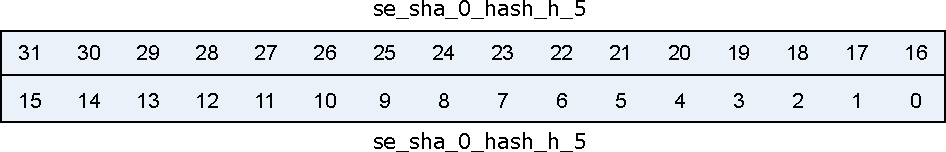
\includegraphics{sec_eng_se_sha_0_hash_h_5.pdf}
\end{figure}

\regdes{31:0&se\_sha\_0\_hash\_h\_5&r&0&big-endian hash 5\\\hline

}
\subsection{se\_sha\_0\_hash\_h\_6}
\label{sec_eng-se-sha-0-hash-h-6}
Address:0x20004048
 \begin{figure}[H]
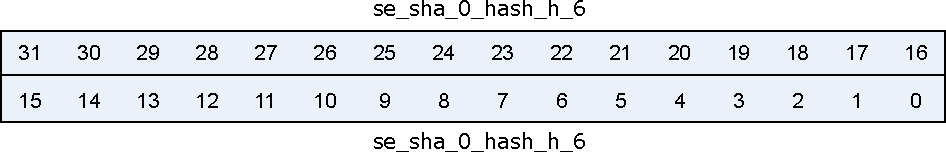
\includegraphics{sec_eng_se_sha_0_hash_h_6.pdf}
\end{figure}

\regdes{31:0&se\_sha\_0\_hash\_h\_6&r&0&big-endian hash 6\\\hline

}
\subsection{se\_sha\_0\_hash\_h\_7}
\label{sec_eng-se-sha-0-hash-h-7}
Address:0x2000404c
 \begin{figure}[H]
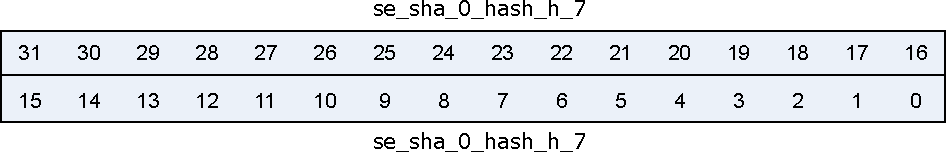
\includegraphics{sec_eng_se_sha_0_hash_h_7.pdf}
\end{figure}

\regdes{31:0&se\_sha\_0\_hash\_h\_7&r&0&big-endian hash 7 (LSB)\\\hline

}
\subsection{se\_sha\_0\_link}
\label{sec_eng-se-sha-0-link}
Address:0x20004050
 \begin{figure}[H]
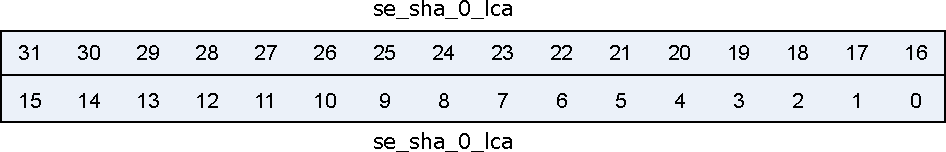
\includegraphics{sec_eng_se_sha_0_link.pdf}
\end{figure}

\regdes{31:0&se\_sha\_0\_lca&r/w&0&aes link config address(word align)\\\hline

}
\subsection{se\_sha\_0\_ctrl\_prot}
\label{sec_eng-se-sha-0-ctrl-prot}
Address:0x200040fc
 \begin{figure}[H]
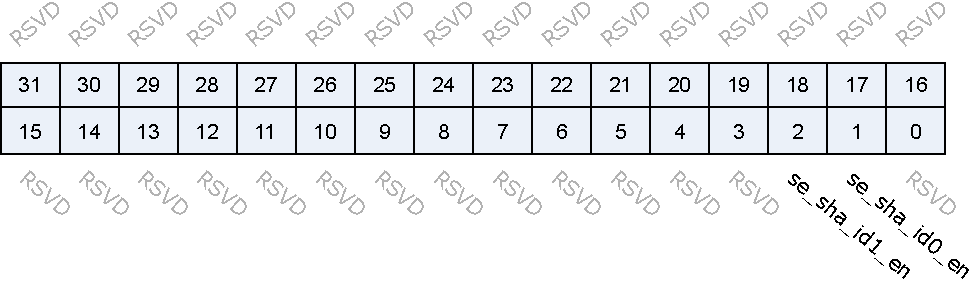
\includegraphics{sec_eng_se_sha_0_ctrl_prot.pdf}
\end{figure}

\regdes{31:3&RSVD& & & \\\hline
2&se\_sha\_id1\_en&r/w&1&id1 access right\\\hline
1&se\_sha\_id0\_en&r/w&1&id0 access right\\\hline
0&RSVD& & & \\\hline

}
\subsection{se\_aes\_0\_ctrl}
\label{sec_eng-se-aes-0-ctrl}
Address:0x20004100
 \begin{figure}[H]
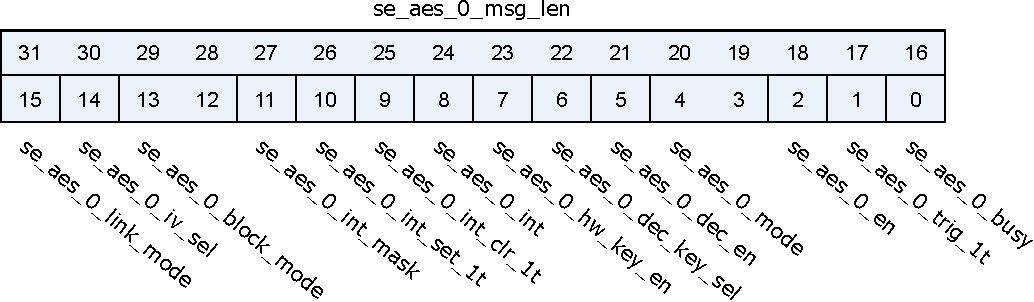
\includegraphics{sec_eng_se_aes_0_ctrl.pdf}
\end{figure}

\regdes{31:16&se\_aes\_0\_msg\_len&r/w&0&number of 128-bit block\\\hline
15&se\_aes\_0\_link\_mode&r/w&0&1:enable aes link mode\\\hline
14&se\_aes\_0\_iv\_sel&r/w&0&0:new iv 1:same iv as last one\\\hline
13:12&se\_aes\_0\_block\_mode&r/w&0&0:ECB mode 1:CTR mode 2:CBC mode 3:XTS mode\\\hline
11&se\_aes\_0\_int\_mask&r/w&0&\\\hline
10&se\_aes\_0\_int\_set\_1t&w1p&0&1:set interrupt\\\hline
9&se\_aes\_0\_int\_clr\_1t&w1p&0&1:clear interrupt\\\hline
8&se\_aes\_0\_int&r&0&interrupt value\\\hline
7&se\_aes\_0\_hw\_key\_en&r/w&0&0:sw key 1:hw key\\\hline
6&se\_aes\_0\_dec\_key\_sel&r/w&0&0:new key 1:same key as last one\\\hline
5&se\_aes\_0\_dec\_en&r/w&0&0:encode 1:decode\\\hline
4:3&se\_aes\_0\_mode&r/w&0&0:128-bit mode 1:256-bit mode 2:192-bit mode 3:128-bit double key mode\\\hline
2&se\_aes\_0\_en&r/w&0&0:disable 1:enable aes\\\hline
1&se\_aes\_0\_trig\_1t&w1p&0&1:trigger aes engine\\\hline
0&se\_aes\_0\_busy&r&0&1:aes engine busy\\\hline

}
\subsection{se\_aes\_0\_msa}
\label{sec_eng-se-aes-0-msa}
Address:0x20004104
 \begin{figure}[H]
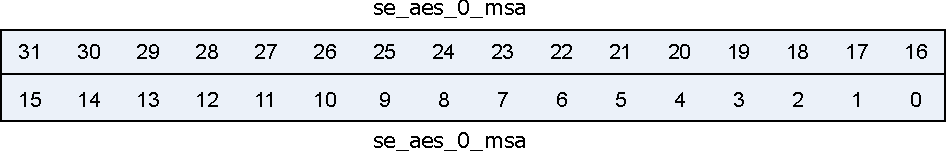
\includegraphics{sec_eng_se_aes_0_msa.pdf}
\end{figure}

\regdes{31:0&se\_aes\_0\_msa&r/w&0&message source address\\\hline

}
\subsection{se\_aes\_0\_mda}
\label{sec_eng-se-aes-0-mda}
Address:0x20004108
 \begin{figure}[H]
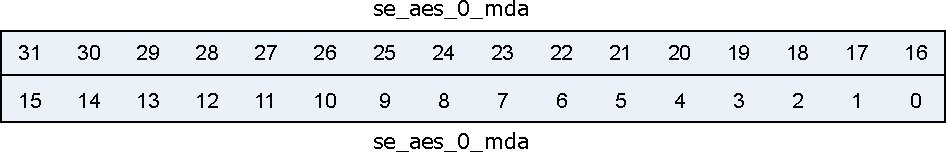
\includegraphics{sec_eng_se_aes_0_mda.pdf}
\end{figure}

\regdes{31:0&se\_aes\_0\_mda&r/w&0&message destination address\\\hline

}
\subsection{se\_aes\_0\_status}
\label{sec_eng-se-aes-0-status}
Address:0x2000410c
 \begin{figure}[H]
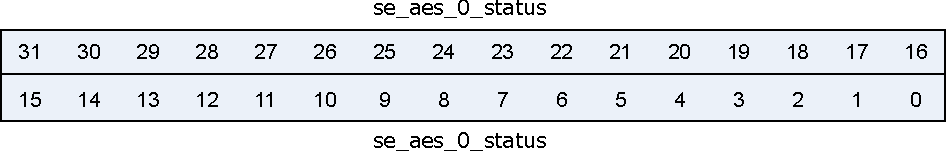
\includegraphics{sec_eng_se_aes_0_status.pdf}
\end{figure}

\regdes{31:0&se\_aes\_0\_status&r&32'h4100&\\\hline

}
\subsection{se\_aes\_0\_iv\_0}
\label{sec_eng-se-aes-0-iv-0}
Address:0x20004110
 \begin{figure}[H]
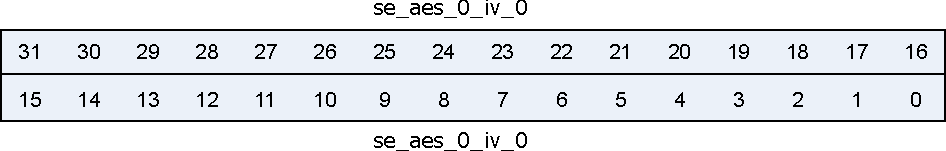
\includegraphics{sec_eng_se_aes_0_iv_0.pdf}
\end{figure}

\regdes{31:0&se\_aes\_0\_iv\_0&r/w&0&big endian initial vector (MSB)\\\hline

}
\subsection{se\_aes\_0\_iv\_1}
\label{sec_eng-se-aes-0-iv-1}
Address:0x20004114
 \begin{figure}[H]
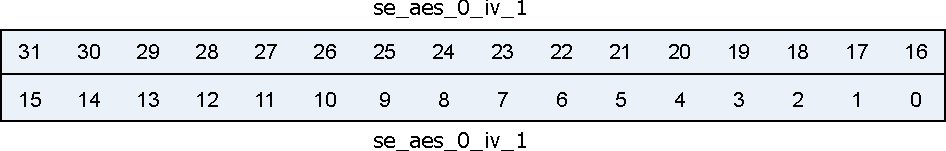
\includegraphics{sec_eng_se_aes_0_iv_1.pdf}
\end{figure}

\regdes{31:0&se\_aes\_0\_iv\_1&r/w&0&big endian initial vector\\\hline

}
\subsection{se\_aes\_0\_iv\_2}
\label{sec_eng-se-aes-0-iv-2}
Address:0x20004118
 \begin{figure}[H]
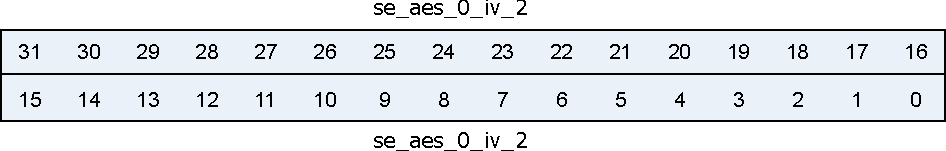
\includegraphics{sec_eng_se_aes_0_iv_2.pdf}
\end{figure}

\regdes{31:0&se\_aes\_0\_iv\_2&r/w&0&big endian initial vector\\\hline

}
\subsection{se\_aes\_0\_iv\_3}
\label{sec_eng-se-aes-0-iv-3}
Address:0x2000411c
 \begin{figure}[H]
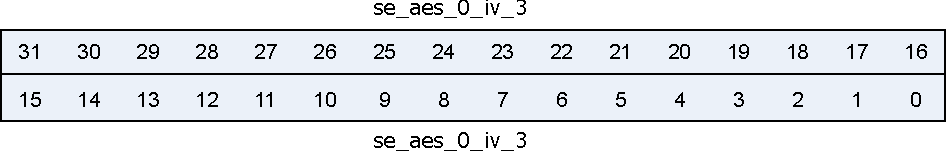
\includegraphics{sec_eng_se_aes_0_iv_3.pdf}
\end{figure}

\regdes{31:0&se\_aes\_0\_iv\_3&r/w&0&big endian initial vector (LSB) (CTR mode: 32-bit counter initial value)\\\hline

}
\subsection{se\_aes\_0\_key\_0}
\label{sec_eng-se-aes-0-key-0}
Address:0x20004120
 \begin{figure}[H]
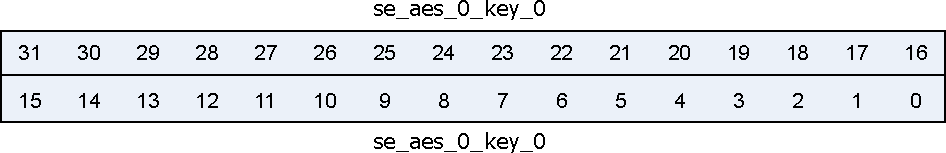
\includegraphics{sec_eng_se_aes_0_key_0.pdf}
\end{figure}

\regdes{31:0&se\_aes\_0\_key\_0&r/w&0&big endian aes key (aes-128/256 key MSB)\\\hline

}
\subsection{se\_aes\_0\_key\_1}
\label{sec_eng-se-aes-0-key-1}
Address:0x20004124
 \begin{figure}[H]
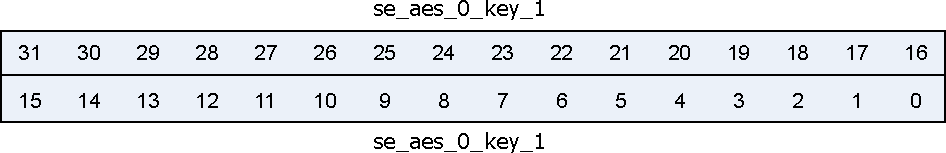
\includegraphics{sec_eng_se_aes_0_key_1.pdf}
\end{figure}

\regdes{31:0&se\_aes\_0\_key\_1&r/w&0&big endian aes key\\\hline

}
\subsection{se\_aes\_0\_key\_2}
\label{sec_eng-se-aes-0-key-2}
Address:0x20004128
 \begin{figure}[H]
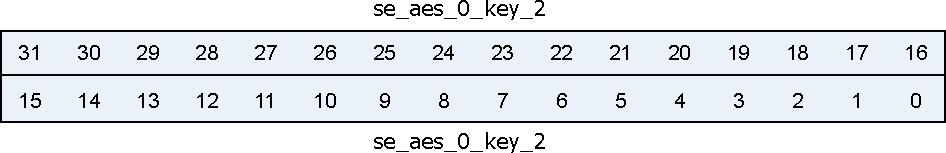
\includegraphics{sec_eng_se_aes_0_key_2.pdf}
\end{figure}

\regdes{31:0&se\_aes\_0\_key\_2&r/w&0&big endian aes key\\\hline

}
\subsection{se\_aes\_0\_key\_3}
\label{sec_eng-se-aes-0-key-3}
Address:0x2000412c
 \begin{figure}[H]
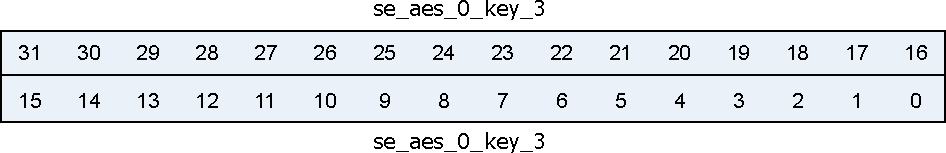
\includegraphics{sec_eng_se_aes_0_key_3.pdf}
\end{figure}

\regdes{31:0&se\_aes\_0\_key\_3&r/w&0&big endian aes key (aes-128 key LSB)\\\hline

}
\subsection{se\_aes\_0\_key\_4}
\label{sec_eng-se-aes-0-key-4}
Address:0x20004130
 \begin{figure}[H]
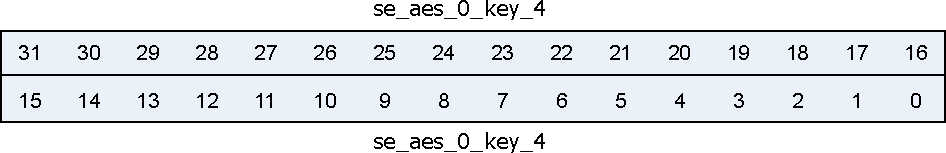
\includegraphics{sec_eng_se_aes_0_key_4.pdf}
\end{figure}

\regdes{31:0&se\_aes\_0\_key\_4&r/w&0&big endian aes key\\\hline

}
\subsection{se\_aes\_0\_key\_5}
\label{sec_eng-se-aes-0-key-5}
Address:0x20004134
 \begin{figure}[H]
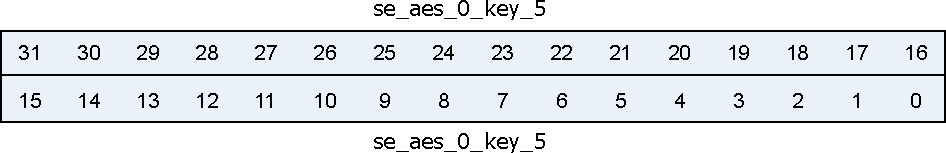
\includegraphics{sec_eng_se_aes_0_key_5.pdf}
\end{figure}

\regdes{31:0&se\_aes\_0\_key\_5&r/w&0&big endian aes key\\\hline

}
\subsection{se\_aes\_0\_key\_6}
\label{sec_eng-se-aes-0-key-6}
Address:0x20004138
 \begin{figure}[H]
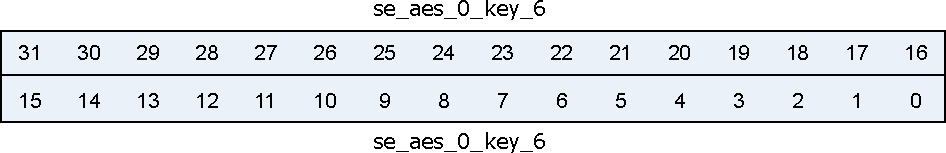
\includegraphics{sec_eng_se_aes_0_key_6.pdf}
\end{figure}

\regdes{31:0&se\_aes\_0\_key\_6&r/w&0&big endian aes key\\\hline

}
\subsection{se\_aes\_0\_key\_7}
\label{sec_eng-se-aes-0-key-7}
Address:0x2000413c
 \begin{figure}[H]
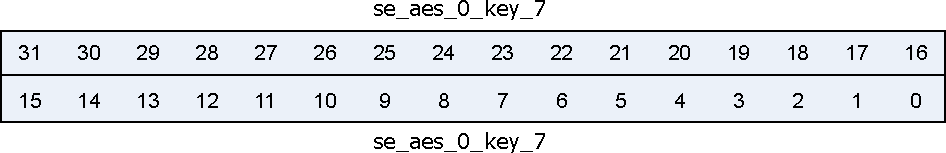
\includegraphics{sec_eng_se_aes_0_key_7.pdf}
\end{figure}

\regdes{31:0&se\_aes\_0\_key\_7&r/w&0&big endian aes key (aes-256 key LSB)\\\hline

}
\subsection{se\_aes\_0\_key\_sel}
\label{sec_eng-se-aes-0-key-sel}
Address:0x20004140
 \begin{figure}[H]
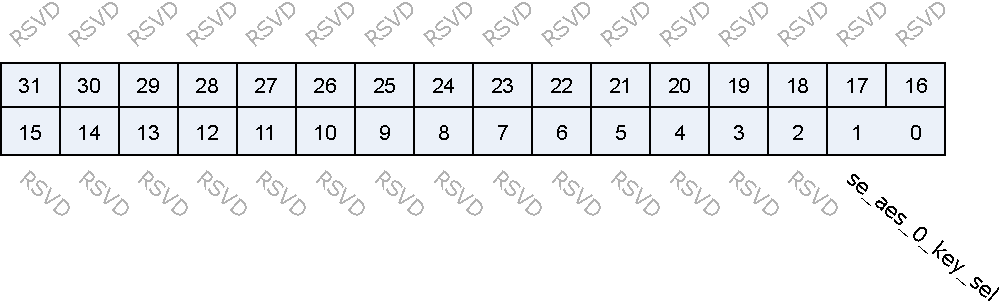
\includegraphics{sec_eng_se_aes_0_key_sel.pdf}
\end{figure}

\regdes{31:2&RSVD& & & \\\hline
1:0&se\_aes\_0\_key\_sel&r/w&0&\\\hline

}
\subsection{se\_aes\_1\_key\_sel}
\label{sec_eng-se-aes-1-key-sel}
Address:0x20004144
 \begin{figure}[H]
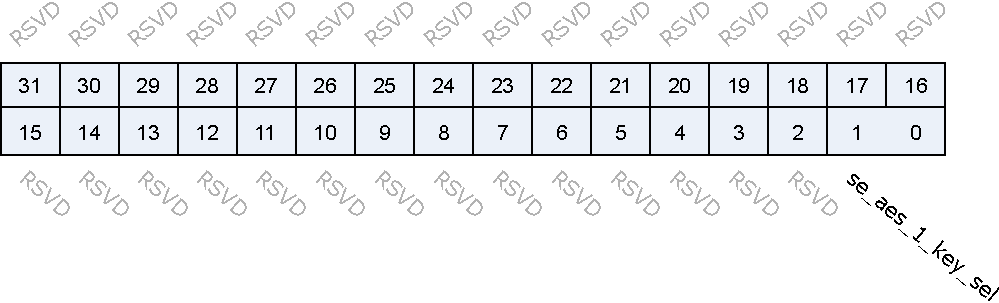
\includegraphics{sec_eng_se_aes_1_key_sel.pdf}
\end{figure}

\regdes{31:2&RSVD& & & \\\hline
1:0&se\_aes\_1\_key\_sel&r/w&0&\\\hline

}
\subsection{se\_aes\_0\_endian}
\label{sec_eng-se-aes-0-endian}
Address:0x20004148
 \begin{figure}[H]
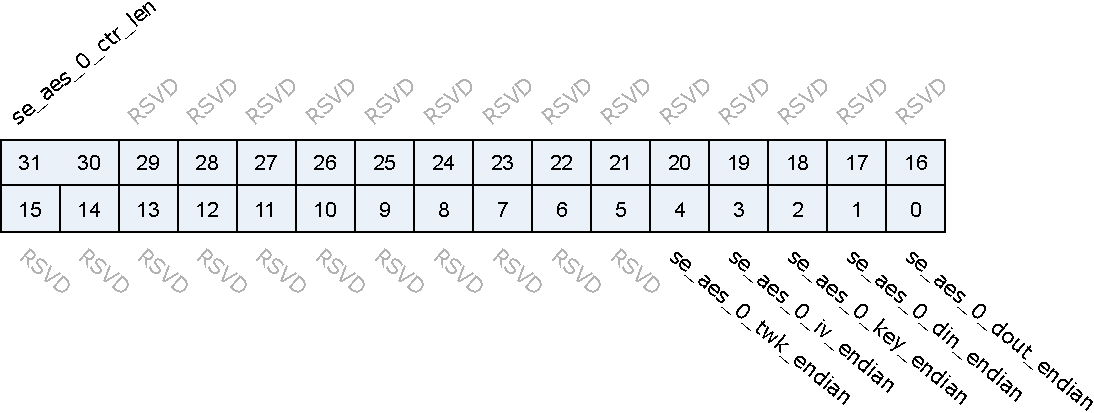
\includegraphics{sec_eng_se_aes_0_endian.pdf}
\end{figure}

\regdes{31:30&se\_aes\_0\_ctr\_len&r/w&0&2'd0:4-byte counter, 2'd1:1-byte counter, 2'd2:2-byte counter, 2'd3:3-byte counter\\\hline
29:5&RSVD& & & \\\hline
4&se\_aes\_0\_twk\_endian&r/w&1&0:little-endian 1:big-endian, default 1 for XTS\\\hline
3&se\_aes\_0\_iv\_endian&r/w&1&0:little-endian 1:big-endian\\\hline
2&se\_aes\_0\_key\_endian&r/w&1&0:little-endian 1:big-endian\\\hline
1&se\_aes\_0\_din\_endian&r/w&1&0:little-endian 1:big-endian\\\hline
0&se\_aes\_0\_dout\_endian&r/w&1&0:little-endian 1:big-endian\\\hline

}
\subsection{se\_aes\_sboot}
\label{sec_eng-se-aes-sboot}
Address:0x2000414c
 \begin{figure}[H]
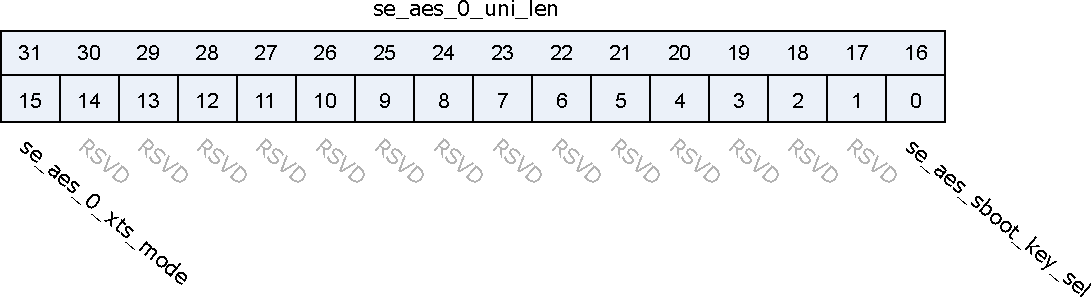
\includegraphics{sec_eng_se_aes_sboot.pdf}
\end{figure}

\regdes{31:16&se\_aes\_0\_uni\_len&r/w&16'd2&XTS data unit length: number of 128-bit blocks in a data unit, msg\_len = N*uni\_len\\\hline
15&se\_aes\_0\_xts\_mode&r/w&0&0: normal XTS, 1: XTS with only one data unit\\\hline
14:1&RSVD& & & \\\hline
0&se\_aes\_sboot\_key\_sel&r/w&0&\\\hline

}
\subsection{se\_aes\_0\_link}
\label{sec_eng-se-aes-0-link}
Address:0x20004150
 \begin{figure}[H]
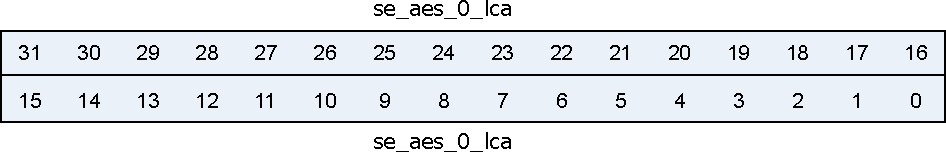
\includegraphics{sec_eng_se_aes_0_link.pdf}
\end{figure}

\regdes{31:0&se\_aes\_0\_lca&r/w&0&aes link config address(word align)\\\hline

}
\subsection{se\_aes\_0\_ctrl\_prot}
\label{sec_eng-se-aes-0-ctrl-prot}
Address:0x200041fc
 \begin{figure}[H]
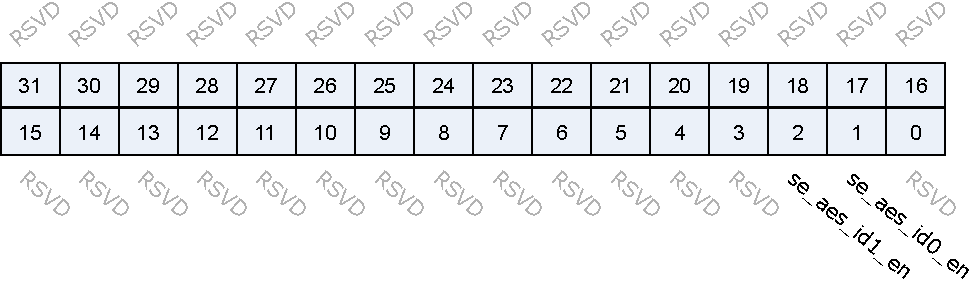
\includegraphics{sec_eng_se_aes_0_ctrl_prot.pdf}
\end{figure}

\regdes{31:3&RSVD& & & \\\hline
2&se\_aes\_id1\_en&r/w&1&id1 access right\\\hline
1&se\_aes\_id0\_en&r/w&1&id0 access right\\\hline
0&RSVD& & & \\\hline

}
\subsection{se\_trng\_0\_ctrl\_0}
\label{sec_eng-se-trng-0-ctrl-0}
Address:0x20004200
 \begin{figure}[H]
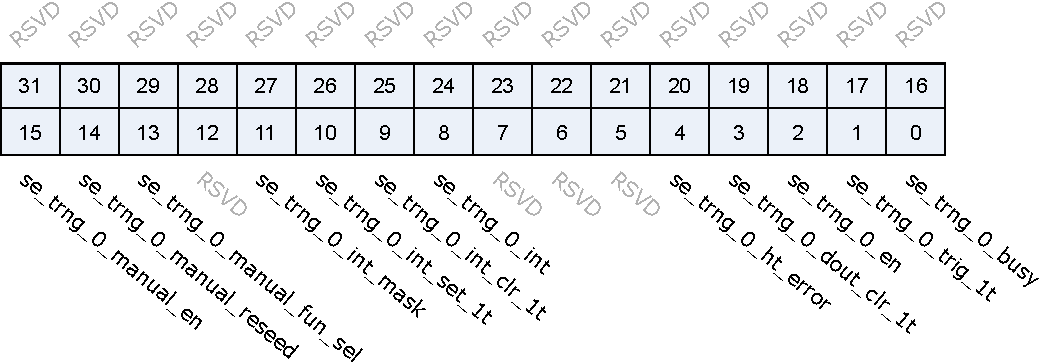
\includegraphics{sec_eng_se_trng_0_ctrl_0.pdf}
\end{figure}

\regdes{31:16&RSVD& & & \\\hline
15&se\_trng\_0\_manual\_en&r/w&0&1:enable manual mode\\\hline
14&se\_trng\_0\_manual\_reseed&r/w&0&1:clear reseed counter to zero and get new entropy\\\hline
13&se\_trng\_0\_manual\_fun\_sel&r/w&0&0:go to instantiate state 1:go to generate state\\\hline
12&RSVD& & & \\\hline
11&se\_trng\_0\_int\_mask&r/w&0&\\\hline
10&se\_trng\_0\_int\_set\_1t&w1p&0&1:set interrupt\\\hline
9&se\_trng\_0\_int\_clr\_1t&w1p&0&1:clear interrupt\\\hline
8&se\_trng\_0\_int&r&0&interrupt value\\\hline
7:5&RSVD& & & \\\hline
4&se\_trng\_0\_ht\_error&r&0&1:health test error\\\hline
3&se\_trng\_0\_dout\_clr\_1t&w1p&0&1:clear trng dout to zero\\\hline
2&se\_trng\_0\_en&r/w&0&0:disable 1:enable aes\\\hline
1&se\_trng\_0\_trig\_1t&w1p&0&1:trigger trng engine\\\hline
0&se\_trng\_0\_busy&r&0&1:trng engine busy\\\hline

}
\subsection{se\_trng\_0\_status}
\label{sec_eng-se-trng-0-status}
Address:0x20004204
 \begin{figure}[H]
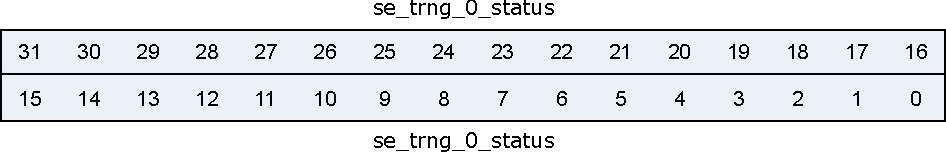
\includegraphics{sec_eng_se_trng_0_status.pdf}
\end{figure}

\regdes{31:0&se\_trng\_0\_status&r&32'h100020&\\\hline

}
\subsection{se\_trng\_0\_dout\_0}
\label{sec_eng-se-trng-0-dout-0}
Address:0x20004208
 \begin{figure}[H]
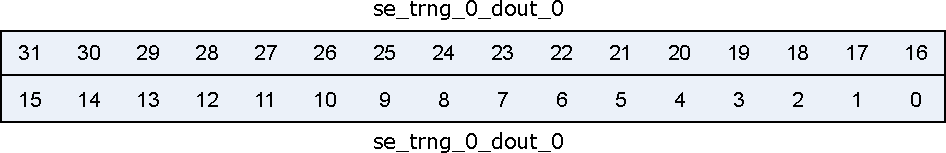
\includegraphics{sec_eng_se_trng_0_dout_0.pdf}
\end{figure}

\regdes{31:0&se\_trng\_0\_dout\_0&r&0&random value\\\hline

}
\subsection{se\_trng\_0\_dout\_1}
\label{sec_eng-se-trng-0-dout-1}
Address:0x2000420c
 \begin{figure}[H]
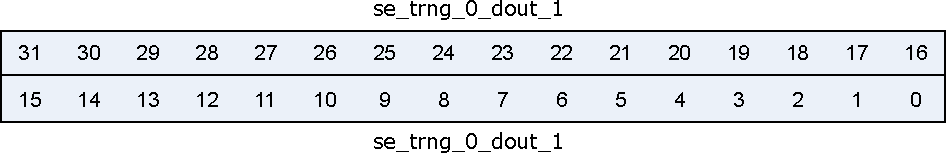
\includegraphics{sec_eng_se_trng_0_dout_1.pdf}
\end{figure}

\regdes{31:0&se\_trng\_0\_dout\_1&r&0&random value\\\hline

}
\subsection{se\_trng\_0\_dout\_2}
\label{sec_eng-se-trng-0-dout-2}
Address:0x20004210
 \begin{figure}[H]
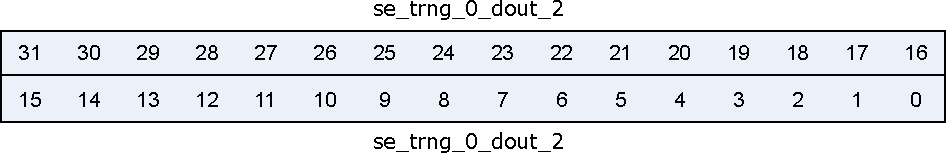
\includegraphics{sec_eng_se_trng_0_dout_2.pdf}
\end{figure}

\regdes{31:0&se\_trng\_0\_dout\_2&r&0&random value\\\hline

}
\subsection{se\_trng\_0\_dout\_3}
\label{sec_eng-se-trng-0-dout-3}
Address:0x20004214
 \begin{figure}[H]
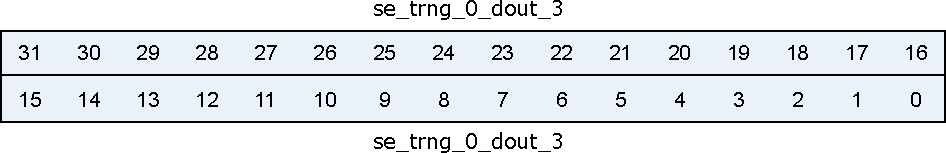
\includegraphics{sec_eng_se_trng_0_dout_3.pdf}
\end{figure}

\regdes{31:0&se\_trng\_0\_dout\_3&r&0&random value\\\hline

}
\subsection{se\_trng\_0\_dout\_4}
\label{sec_eng-se-trng-0-dout-4}
Address:0x20004218
 \begin{figure}[H]
\includegraphics{sec_eng_se_trng_0_dout_4.pdf}
\end{figure}

\regdes{31:0&se\_trng\_0\_dout\_4&r&0&random value\\\hline

}
\subsection{se\_trng\_0\_dout\_5}
\label{sec_eng-se-trng-0-dout-5}
Address:0x2000421c
 \begin{figure}[H]
\includegraphics{sec_eng_se_trng_0_dout_5.pdf}
\end{figure}

\regdes{31:0&se\_trng\_0\_dout\_5&r&0&random value\\\hline

}
\subsection{se\_trng\_0\_dout\_6}
\label{sec_eng-se-trng-0-dout-6}
Address:0x20004220
 \begin{figure}[H]
\includegraphics{sec_eng_se_trng_0_dout_6.pdf}
\end{figure}

\regdes{31:0&se\_trng\_0\_dout\_6&r&0&random value\\\hline

}
\subsection{se\_trng\_0\_dout\_7}
\label{sec_eng-se-trng-0-dout-7}
Address:0x20004224
 \begin{figure}[H]
\includegraphics{sec_eng_se_trng_0_dout_7.pdf}
\end{figure}

\regdes{31:0&se\_trng\_0\_dout\_7&r&0&random value\\\hline

}
\subsection{se\_trng\_0\_test}
\label{sec_eng-se-trng-0-test}
Address:0x20004228
 \begin{figure}[H]
\includegraphics{sec_eng_se_trng_0_test.pdf}
\end{figure}

\regdes{31:12&RSVD& & & \\\hline
11:4&se\_trng\_0\_ht\_alarm\_n&r/w&8'd0&health test alarm number \par 0:alarm if health test error >= 1 \par 1:alarm if health test error >= 2
\\\hline
3&se\_trng\_0\_ht\_dis&r/w&0&1:disable health test\\\hline
2&se\_trng\_0\_cp\_bypass&r/w&0&1:bypass conditional component\\\hline
1&se\_trng\_0\_cp\_test\_en&r/w&0&1:enable trng conditional component test mode\\\hline
0&se\_trng\_0\_test\_en&r/w&0&1:enable trng test mode\\\hline

}
\subsection{se\_trng\_0\_ctrl\_1}
\label{sec_eng-se-trng-0-ctrl-1}
Address:0x2000422c
 \begin{figure}[H]
\includegraphics{sec_eng_se_trng_0_ctrl_1.pdf}
\end{figure}

\regdes{31:0&se\_trng\_0\_reseed\_n\_lsb&r/w&32'hffff&reload seed when number of used random value is larger than reseed\_n\\\hline

}
\subsection{se\_trng\_0\_ctrl\_2}
\label{sec_eng-se-trng-0-ctrl-2}
Address:0x20004230
 \begin{figure}[H]
\includegraphics{sec_eng_se_trng_0_ctrl_2.pdf}
\end{figure}

\regdes{31:16&RSVD& & & \\\hline
15:0&se\_trng\_0\_reseed\_n\_msb&r/w&16'hff&reload seed when number of used random value is larger than reseed\_n\\\hline

}
\subsection{se\_trng\_0\_ctrl\_3}
\label{sec_eng-se-trng-0-ctrl-3}
Address:0x20004234
 \begin{figure}[H]
\includegraphics{sec_eng_se_trng_0_ctrl_3.pdf}
\end{figure}

\regdes{31&se\_trng\_0\_rosc\_en&r/w&0&trng rosc enable\\\hline
30:27&RSVD& & & \\\hline
26&se\_trng\_0\_ht\_od\_en&r/w&0&health test on demand test enable\\\hline
25:16&se\_trng\_0\_ht\_apt\_c&r/w&10'd890&health test adaptive proportion test cut off value\\\hline
15:8&se\_trng\_0\_ht\_rct\_c&r/w&8'd66&health test repetition count test cut off value\\\hline
7:0&se\_trng\_0\_cp\_ratio&r/w&8'd3&conditional component compression ration\\\hline

}
\subsection{se\_trng\_0\_test\_out\_0}
\label{sec_eng-se-trng-0-test-out-0}
Address:0x20004240
 \begin{figure}[H]
\includegraphics{sec_eng_se_trng_0_test_out_0.pdf}
\end{figure}

\regdes{31:0&se\_trng\_0\_test\_out\_0&r&0&\\\hline

}
\subsection{se\_trng\_0\_test\_out\_1}
\label{sec_eng-se-trng-0-test-out-1}
Address:0x20004244
 \begin{figure}[H]
\includegraphics{sec_eng_se_trng_0_test_out_1.pdf}
\end{figure}

\regdes{31:0&se\_trng\_0\_test\_out\_1&r&0&\\\hline

}
\subsection{se\_trng\_0\_test\_out\_2}
\label{sec_eng-se-trng-0-test-out-2}
Address:0x20004248
 \begin{figure}[H]
\includegraphics{sec_eng_se_trng_0_test_out_2.pdf}
\end{figure}

\regdes{31:0&se\_trng\_0\_test\_out\_2&r&0&\\\hline

}
\subsection{se\_trng\_0\_test\_out\_3}
\label{sec_eng-se-trng-0-test-out-3}
Address:0x2000424c
 \begin{figure}[H]
\includegraphics{sec_eng_se_trng_0_test_out_3.pdf}
\end{figure}

\regdes{31:0&se\_trng\_0\_test\_out\_3&r&0&\\\hline

}
\subsection{se\_trng\_0\_ctrl\_prot}
\label{sec_eng-se-trng-0-ctrl-prot}
Address:0x200042fc
 \begin{figure}[H]
\includegraphics{sec_eng_se_trng_0_ctrl_prot.pdf}
\end{figure}

\regdes{31:3&RSVD& & & \\\hline
2&se\_trng\_id1\_en&r/w&1&id1 access right\\\hline
1&se\_trng\_id0\_en&r/w&1&id0 access right\\\hline
0&RSVD& & & \\\hline

}
\subsection{se\_pka\_0\_ctrl\_0}
\label{sec_eng-se-pka-0-ctrl-0}
Address:0x20004300
 \begin{figure}[H]
\includegraphics{sec_eng_se_pka_0_ctrl_0.pdf}
\end{figure}

\regdes{31:16&se\_pka\_0\_status&r&0&[31]cmd\_err, \par [30:26]cmd\_err\_idx[4:0] \par [25]opq\_full, \par [24]last\_opc, \par [23]err\_cam\_full, \par [22]err\_div\_by\_0, \par [21]err\_invalid\_src0 \par [20]err\_invalid\_src1 \par [19]err\_invalid\_src2 \par [18]err\_opq\_overflow \par [17]err\_unknown\_opc \par [16]prime\_fail
\\\hline
15&se\_pka\_0\_status\_clr\_1t&w1p&0&\\\hline
14&RSVD& & & \\\hline
13&se\_pka\_0\_ram\_clr\_md&r/w&0&\\\hline
12&se\_pka\_0\_endian&r/w&0&\\\hline
11&se\_pka\_0\_int\_mask&r/w&0&\\\hline
10&se\_pka\_0\_int\_set&r/w&0&1:set interrupt\\\hline
9&se\_pka\_0\_int\_clr\_1t&w1p&0&1:clear interrupt\\\hline
8&se\_pka\_0\_int&r&0&interrupt value\\\hline
7:4&se\_pka\_0\_prot\_md&r/w&0&\\\hline
3&se\_pka\_0\_en&r/w&0&\\\hline
2&se\_pka\_0\_busy&r&0&\\\hline
1&se\_pka\_0\_done\_clr\_1t&w1p&0&\\\hline
0&se\_pka\_0\_done&r&0&\\\hline

}
\subsection{se\_pka\_0\_seed}
\label{sec_eng-se-pka-0-seed}
Address:0x2000430c
 \begin{figure}[H]
\includegraphics{sec_eng_se_pka_0_seed.pdf}
\end{figure}

\regdes{31:0&se\_pka\_0\_seed&r/w&0&\\\hline

}
\subsection{se\_pka\_0\_ctrl\_1}
\label{sec_eng-se-pka-0-ctrl-1}
Address:0x20004310
 \begin{figure}[H]
\includegraphics{sec_eng_se_pka_0_ctrl_1.pdf}
\end{figure}

\regdes{31:4&RSVD& & & \\\hline
3&se\_pka\_0\_hbypass&r/w&0&\\\hline
2:0&se\_pka\_0\_hburst&r/w&3'd5&3'b000:single \par 3'b001:incr (undefined length) \par 3'b010:4-beat wrap \par 3'b011:4-beat incr \par 3'b100:8-beat wrap \par 3'b101:8-beat incr(default)
\\\hline

}
\subsection{se\_pka\_0\_rw}
\label{sec_eng-se-pka-0-rw}
Address:0x20004340
 \begin{figure}[H]
\includegraphics{sec_eng_se_pka_0_rw.pdf}
\end{figure}

\regdes{31:0&se\_pka\_0\_rw&r/w&0&0x340~0x35F single write for command\\\hline

}
\subsection{se\_pka\_0\_rw\_burst}
\label{sec_eng-se-pka-0-rw-burst}
Address:0x20004360
 \begin{figure}[H]
\includegraphics{sec_eng_se_pka_0_rw_burst.pdf}
\end{figure}

\regdes{31:0&se\_pka\_0\_rw\_burst&r/w&0&0x360~0x37F burst write for data\\\hline

}
\subsection{se\_pka\_0\_ctrl\_prot}
\label{sec_eng-se-pka-0-ctrl-prot}
Address:0x200043fc
 \begin{figure}[H]
\includegraphics{sec_eng_se_pka_0_ctrl_prot.pdf}
\end{figure}

\regdes{31:3&RSVD& & & \\\hline
2&se\_pka\_id1\_en&r/w&1&id1 access right\\\hline
1&se\_pka\_id0\_en&r/w&1&id0 access right\\\hline
0&RSVD& & & \\\hline

}
\subsection{se\_cdet\_0\_ctrl\_0}
\label{sec_eng-se-cdet-0-ctrl-0}
Address:0x20004400
 \begin{figure}[H]
\includegraphics{sec_eng_se_cdet_0_ctrl_0.pdf}
\end{figure}

\regdes{31:13&RSVD& & & \\\hline
12&se\_cdet\_0\_mode&r/w&0&1:clock detection manual mode for sw usage\\\hline
11&se\_cdet\_0\_int\_mask&r/w&0&\\\hline
10&se\_cdet\_0\_int\_set&r/w&0&1:set interrupt\\\hline
9&se\_cdet\_0\_int\_clr&r/w&0&1:clear interrupt\\\hline
8&se\_cdet\_0\_int&r&0&interrupt value\\\hline
7:3&se\_cdet\_0\_status&r&1&\\\hline
2&RSVD& & & \\\hline
1&se\_cdet\_0\_busy&r&0&\\\hline
0&se\_cdet\_0\_en&r/w&0&\\\hline

}
\subsection{se\_cdet\_0\_ctrl\_1}
\label{sec_eng-se-cdet-0-ctrl-1}
Address:0x20004404
 \begin{figure}[H]
\includegraphics{sec_eng_se_cdet_0_ctrl_1.pdf}
\end{figure}

\regdes{31:16&se\_cdet\_0\_g\_loop\_min&r/w&16'd33&\\\hline
15:0&se\_cdet\_0\_g\_loop\_max&r/w&16'd100&\\\hline

}
\subsection{se\_cdet\_0\_ctrl\_2}
\label{sec_eng-se-cdet-0-ctrl-2}
Address:0x20004408
 \begin{figure}[H]
\includegraphics{sec_eng_se_cdet_0_ctrl_2.pdf}
\end{figure}

\regdes{31:24&se\_cdet\_0\_g\_slp\_n&r/w&8'd255&\\\hline
23:16&se\_cdet\_0\_t\_dly\_n&r/w&8'd3&\\\hline
15:0&se\_cdet\_0\_t\_loop\_n&r/w&16'd50&\\\hline

}
\subsection{se\_cdet\_0\_ctrl\_3}
\label{sec_eng-se-cdet-0-ctrl-3}
Address:0x2000440c
 \begin{figure}[H]
\includegraphics{sec_eng_se_cdet_0_ctrl_3.pdf}
\end{figure}

\regdes{31:16&se\_cdet\_0\_g\_count&r&0&\\\hline
15:0&se\_cdet\_0\_t\_count&r&0&\\\hline

}
\subsection{se\_cdet\_0\_ctrl\_prot}
\label{sec_eng-se-cdet-0-ctrl-prot}
Address:0x200044fc
 \begin{figure}[H]
\includegraphics{sec_eng_se_cdet_0_ctrl_prot.pdf}
\end{figure}

\regdes{31:3&RSVD& & & \\\hline
2&se\_cdet\_id1\_en&r/w&1&id1 access right\\\hline
1&se\_cdet\_id0\_en&r/w&1&id0 access right\\\hline
0&se\_cdet\_prot\_en&r/w&1&1:control register protection enable\\\hline

}
\subsection{se\_gmac\_0\_ctrl\_0}
\label{sec_eng-se-gmac-0-ctrl-0}
Address:0x20004500
 \begin{figure}[H]
\includegraphics{sec_eng_se_gmac_0_ctrl_0.pdf}
\end{figure}

\regdes{31:15&RSVD& & & \\\hline
14&se\_gmac\_0\_x\_endian&r/w&1&0:little-endian 1:big-endian\\\hline
13&se\_gmac\_0\_h\_endian&r/w&1&0:little-endian 1:big-endian\\\hline
12&se\_gmac\_0\_t\_endian&r/w&1&0:little-endian 1:big-endian\\\hline
11&se\_gmac\_0\_int\_mask&r/w&0&1:mask interrupt\\\hline
10&se\_gmac\_0\_int\_set\_1t&w1p&0&1:set interrupt\\\hline
9&se\_gmac\_0\_int\_clr\_1t&w1p&0&1:clear interrupt\\\hline
8&se\_gmac\_0\_int&r&0&interrupt value\\\hline
7:3&RSVD& & & \\\hline
2&se\_gmac\_0\_en&r/w&0&0:disable 1:enable gmac\\\hline
1&se\_gmac\_0\_trig\_1t&w1p&0&1:trigger gmac engine\\\hline
0&se\_gmac\_0\_busy&r&0&1:gmac engine busy\\\hline

}
\subsection{se\_gmac\_0\_lca}
\label{sec_eng-se-gmac-0-lca}
Address:0x20004504
 \begin{figure}[H]
\includegraphics{sec_eng_se_gmac_0_lca.pdf}
\end{figure}

\regdes{31:0&se\_gmac\_0\_lca&r/w&0&gmac link config address(word align)\\\hline

}
\subsection{se\_gmac\_0\_status}
\label{sec_eng-se-gmac-0-status}
Address:0x20004508
 \begin{figure}[H]
\includegraphics{sec_eng_se_gmac_0_status.pdf}
\end{figure}

\regdes{31:0&se\_gmac\_0\_status&r&32'hf1000000&\\\hline

}
\subsection{se\_gmac\_0\_ctrl\_prot}
\label{sec_eng-se-gmac-0-ctrl-prot}
Address:0x200045fc
 \begin{figure}[H]
\includegraphics{sec_eng_se_gmac_0_ctrl_prot.pdf}
\end{figure}

\regdes{31:3&RSVD& & & \\\hline
2&se\_gmac\_id1\_en&r/w&1&id1 access right\\\hline
1&se\_gmac\_id0\_en&r/w&1&id0 access right\\\hline
0&RSVD& & & \\\hline

}
\subsection{se\_ctrl\_prot\_rd}
\label{sec_eng-se-ctrl-prot-rd}
Address:0x20004f00
 \begin{figure}[H]
\includegraphics{sec_eng_se_ctrl_prot_rd.pdf}
\end{figure}

\regdes{31&se\_dbg\_dis&r&0&1:disable aes debug mode\\\hline
30:12&RSVD& & & \\\hline
11&se\_gmac\_id1\_en\_rd&r&1&read only status of id1 access right\\\hline
10&se\_gmac\_id0\_en\_rd&r&1&read only status of id0 access right\\\hline
9&se\_cdet\_id1\_en\_rd&r&1&read only status of id1 access right\\\hline
8&se\_cdet\_id0\_en\_rd&r&1&read only status of id0 access right\\\hline
7&se\_pka\_id1\_en\_rd&r&1&read only status of id1 access right\\\hline
6&se\_pka\_id0\_en\_rd&r&1&read only status of id0 access right\\\hline
5&se\_trng\_id1\_en\_rd&r&1&read only status of id1 access right\\\hline
4&se\_trng\_id0\_en\_rd&r&1&read only status of id0 access right\\\hline
3&se\_aes\_id1\_en\_rd&r&1&read only status of id1 access right\\\hline
2&se\_aes\_id0\_en\_rd&r&1&read only status of id0 access right\\\hline
1&se\_sha\_id1\_en\_rd&r&1&read only status of id1 access right\\\hline
0&se\_sha\_id0\_en\_rd&r&1&read only status of id0 access right\\\hline

}
\subsection{se\_ctrl\_reserved\_0}
\label{sec_eng-se-ctrl-reserved-0}
Address:0x20004f04
 \begin{figure}[H]
\includegraphics{sec_eng_se_ctrl_reserved_0.pdf}
\end{figure}

\regdes{31:0&se\_ctrl\_reserved\_0&r/w&0&\\\hline

}
\subsection{se\_ctrl\_reserved\_1}
\label{sec_eng-se-ctrl-reserved-1}
Address:0x20004f08
 \begin{figure}[H]
\includegraphics{sec_eng_se_ctrl_reserved_1.pdf}
\end{figure}

\regdes{31:0&se\_ctrl\_reserved\_1&r/w&32'hffffffff&\\\hline

}
\subsection{se\_ctrl\_reserved\_2}
\label{sec_eng-se-ctrl-reserved-2}
Address:0x20004f0c
 \begin{figure}[H]
\includegraphics{sec_eng_se_ctrl_reserved_2.pdf}
\end{figure}

\regdes{31:0&se\_ctrl\_reserved\_2&r&0&\\\hline

}
